\documentclass[11pt]{article}
\usepackage{tikz}
\usetikzlibrary{positioning}
\tikzstyle{seat} = [rectangle,
                    rounded corners,
                                        minimum width=3cm,
                                                            minimum height=2cm,
                                                                                text centered,
                                                                                                    % node distance=3cm and 1cm,
                                                                                                                        fill=cyan!25,
                                                                                                                                            draw=black]
                                                                                                                                            \begin{document}
                                                                                                                                            \begin{figure}[h]
                                                                                                                                               \centering
                                                                                                                                                  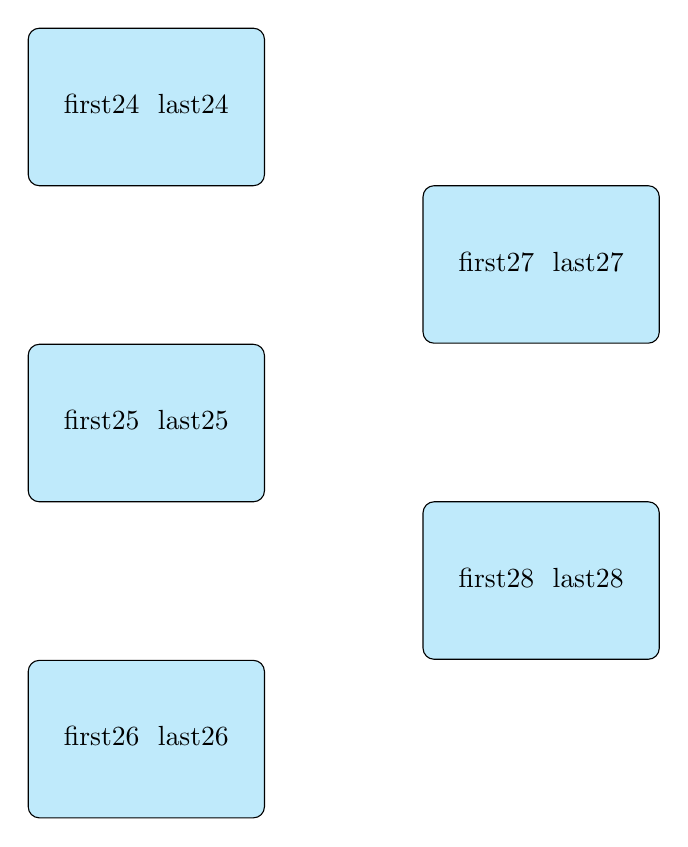
\begin{tikzpicture}[node distance=2cm]
\node (s1) [seat] {\begin{tabular}{c} first24 \ last24 \end{tabular}};
\node (s2) [seat, below= of s1] {\begin{tabular}{c} first25 \ last25 \end{tabular}};
\node (s3) [seat, below= of s2] {\begin{tabular}{c} first26 \ last26 \end{tabular}};
\node (s4) [seat, right= of s1, yshift = -2cm] {\begin{tabular}{c} first27 \ last27 \end{tabular}};
\node (s5) [seat, below= of s4] {\begin{tabular}{c} first28 \ last28 \end{tabular}};
\end{tikzpicture}
\end{figure}
\end{document}